% ============================================================
% Figure Templates for Academic Papers
% ============================================================
% Ready-to-copy TikZ/LaTeX figure templates.
% Requires: \usepackage{tikz, pgfplots, graphicx}
% Optional: \usetikzlibrary{shapes, arrows.meta, positioning, fit, calc}
%
% Replace TODO placeholders with your content.
% ============================================================


% ============================================================
% 1. METHOD OVERVIEW / ARCHITECTURE DIAGRAM
% ============================================================
% Use this for system architecture, model pipeline, or method overview.
% Typically placed as Figure 1 in the paper.

\begin{figure*}[t]
\centering
\begin{tikzpicture}[
    node distance=1.5cm and 2cm,
    block/.style={rectangle, draw, rounded corners, minimum height=1.2cm, minimum width=2.5cm, align=center, fill=blue!8},
    data/.style={rectangle, draw, minimum height=1cm, minimum width=2cm, align=center, fill=green!8},
    output/.style={rectangle, draw, rounded corners, minimum height=1cm, minimum width=2cm, align=center, fill=orange!8},
    arrow/.style={-{Stealth[length=3mm]}, thick},
]
    % Input
    \node[data] (input) {Input\\TODO};

    % Processing blocks
    \node[block, right=of input] (module1) {Module A\\TODO};
    \node[block, right=of module1] (module2) {Module B\\TODO};
    \node[block, right=of module2] (module3) {Module C\\TODO};

    % Output
    \node[output, right=of module3] (output) {Output\\TODO};

    % Arrows
    \draw[arrow] (input) -- (module1);
    \draw[arrow] (module1) -- (module2);
    \draw[arrow] (module2) -- (module3);
    \draw[arrow] (module3) -- (output);

    % Optional: skip connection
    \draw[arrow, dashed, bend left=30] (module1) to node[above, font=\small] {skip} (module3);

    % Optional: labels
    \node[below=0.3cm of module2, font=\small\itshape] {TODO: Overall method name};

\end{tikzpicture}
\caption{Overview of the proposed TODO:METHOD\_NAME. The pipeline consists of TODO:DESCRIPTION. Best viewed in color.}
\label{fig:overview}
\end{figure*}


% ============================================================
% 2. PIPELINE / FLOWCHART
% ============================================================
% Use for data processing pipelines, training workflows, or multi-stage systems.

\begin{figure}[t]
\centering
\begin{tikzpicture}[
    node distance=1.2cm,
    step/.style={rectangle, draw, rounded corners, minimum width=3.5cm, minimum height=0.9cm, align=center, fill=blue!8},
    decision/.style={diamond, draw, aspect=2, minimum width=2cm, align=center, fill=yellow!10},
    arrow/.style={-{Stealth[length=2.5mm]}, thick},
]
    \node[step] (s1) {Step 1: TODO};
    \node[step, below=of s1] (s2) {Step 2: TODO};
    \node[decision, below=of s2] (d1) {TODO\\condition?};
    \node[step, below=of d1] (s3a) {Step 3a: TODO};
    \node[step, right=2.5cm of d1] (s3b) {Step 3b: TODO};
    \node[step, below=of s3a] (s4) {Step 4: TODO};

    \draw[arrow] (s1) -- (s2);
    \draw[arrow] (s2) -- (d1);
    \draw[arrow] (d1) -- node[left, font=\small] {Yes} (s3a);
    \draw[arrow] (d1) -- node[above, font=\small] {No} (s3b);
    \draw[arrow] (s3a) -- (s4);
    \draw[arrow] (s3b) |- (s4);

\end{tikzpicture}
\caption{TODO:PIPELINE\_NAME pipeline. TODO:DESCRIPTION.}
\label{fig:pipeline}
\end{figure}


% ============================================================
% 3. BAR CHART (pgfplots)
% ============================================================
% Use for comparing methods on a single metric.

\begin{figure}[t]
\centering
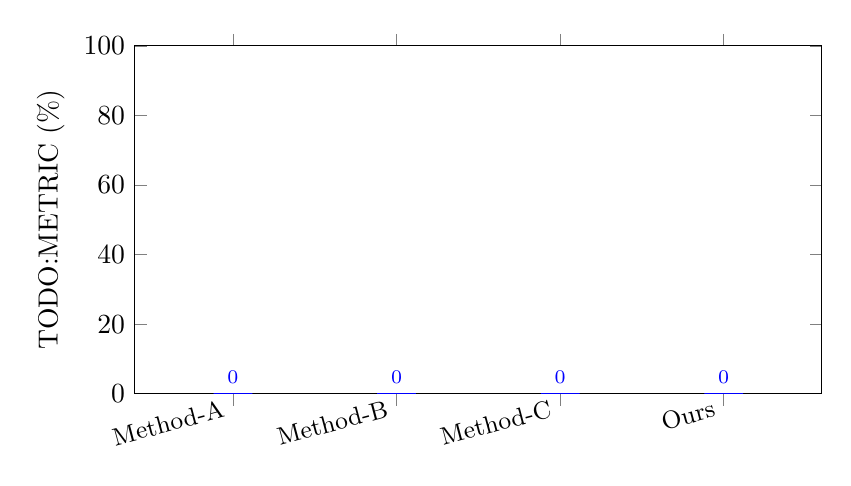
\begin{tikzpicture}
\begin{axis}[
    ybar,
    bar width=14pt,
    ylabel={TODO:METRIC (\%)},
    symbolic x coords={Method-A, Method-B, Method-C, Ours},
    xtick=data,
    x tick label style={rotate=15, anchor=east, font=\small},
    ymin=0, ymax=100,
    nodes near coords,
    nodes near coords align={vertical},
    every node near coord/.append style={font=\scriptsize},
    enlarge x limits=0.2,
    legend style={at={(0.5,1.02)}, anchor=south, legend columns=-1, font=\small},
    width=0.85\columnwidth,
    height=6cm,
]
\addplot coordinates {(Method-A, 0) (Method-B, 0) (Method-C, 0) (Ours, 0)};
% Optional second metric:
% \addplot coordinates {(Method-A, 0) (Method-B, 0) (Method-C, 0) (Ours, 0)};
% \legend{Metric-1, Metric-2}
\end{axis}
\end{tikzpicture}
\caption{Comparison of TODO:METRIC across methods on TODO:DATASET.}
\label{fig:bar_comparison}
\end{figure}


% ============================================================
% 4. LINE CHART (pgfplots)
% ============================================================
% Use for training curves, convergence, or performance vs. parameter.

\begin{figure}[t]
\centering
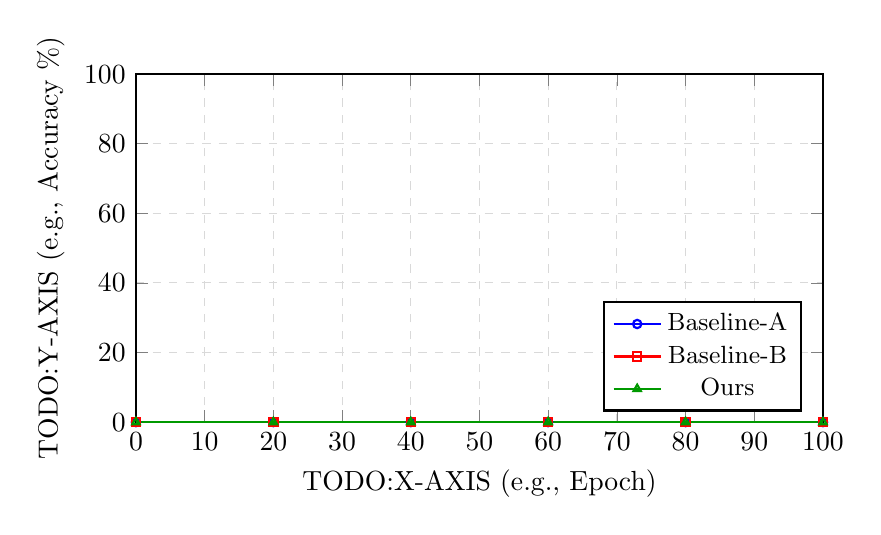
\begin{tikzpicture}
\begin{axis}[
    xlabel={TODO:X-AXIS (e.g., Epoch)},
    ylabel={TODO:Y-AXIS (e.g., Accuracy \%)},
    xmin=0, xmax=100,
    ymin=0, ymax=100,
    legend pos=south east,
    legend style={font=\small},
    grid=major,
    grid style={dashed, gray!30},
    width=0.85\columnwidth,
    height=6cm,
    thick,
]
\addplot[blue, mark=o, mark size=1.5pt] coordinates {
    (0,0) (20,0) (40,0) (60,0) (80,0) (100,0)
};
\addplot[red, mark=square, mark size=1.5pt] coordinates {
    (0,0) (20,0) (40,0) (60,0) (80,0) (100,0)
};
\addplot[green!60!black, mark=triangle, mark size=1.5pt] coordinates {
    (0,0) (20,0) (40,0) (60,0) (80,0) (100,0)
};
\legend{Baseline-A, Baseline-B, Ours}
\end{axis}
\end{tikzpicture}
\caption{TODO:DESCRIPTION over TODO:X-AXIS on TODO:DATASET.}
\label{fig:line_chart}
\end{figure}


% ============================================================
% 5. QUALITATIVE COMPARISON (side-by-side images)
% ============================================================
% Use for visual results: input vs. baseline vs. ours vs. ground truth.

\begin{figure*}[t]
\centering
\setlength{\tabcolsep}{2pt}
\begin{tabular}{cccc}
    \includegraphics[width=0.23\textwidth]{figures/TODO_input.png} &
    \includegraphics[width=0.23\textwidth]{figures/TODO_baseline.png} &
    \includegraphics[width=0.23\textwidth]{figures/TODO_ours.png} &
    \includegraphics[width=0.23\textwidth]{figures/TODO_gt.png} \\
    (a) Input & (b) Baseline & (c) Ours & (d) Ground Truth \\[6pt]
    % Add more rows as needed:
    % \includegraphics[width=0.23\textwidth]{...} & ... \\
    % (a) ... & (b) ... & (c) ... & (d) ... \\
\end{tabular}
\caption{Qualitative comparison on TODO:DATASET. TODO:DESCRIPTION of what the reader should notice.}
\label{fig:qualitative}
\end{figure*}


% ============================================================
% 6. CONFUSION MATRIX / HEATMAP SKELETON
% ============================================================
% Use for classification results. Fill in the matrix values.

\begin{figure}[t]
\centering
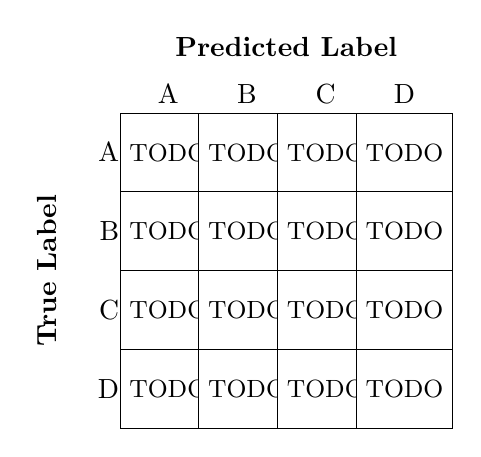
\begin{tikzpicture}[
    cell/.style={minimum size=1cm, align=center, font=\small},
]
    % Labels
    \def\classes{{"A","B","C","D"}}
    \def\nclasses{4}

    % Draw grid
    \foreach \i in {0,...,3} {
        \foreach \j in {0,...,3} {
            \node[cell, draw, fill=blue!\fpeval{0}!white] at (\j+0.5, -\i-0.5) {TODO};
        }
    }

    % Row labels (True)
    \foreach \i in {0,...,3} {
        \pgfmathsetmacro\label{{"A","B","C","D"}[\i]}
        \node[left] at (0, -\i-0.5) {\label};
    }

    % Column labels (Predicted)
    \foreach \j in {0,...,3} {
        \pgfmathsetmacro\label{{"A","B","C","D"}[\j]}
        \node[above] at (\j+0.5, 0) {\label};
    }

    % Axis labels
    \node[rotate=90, anchor=south] at (-0.8, -2) {\textbf{True Label}};
    \node[anchor=south] at (2, 0.6) {\textbf{Predicted Label}};

\end{tikzpicture}
\caption{Confusion matrix of TODO:METHOD on TODO:DATASET.}
\label{fig:confusion}
\end{figure}


% ============================================================
% USAGE NOTES
% ============================================================
% - Always include \label{} for cross-referencing
% - Caption should state the main takeaway, not just describe the figure
% - Use consistent colors across all figures in the paper
% - Check venue rules for figure placement: [t], [h], [b], or figure*
% - Use \textwidth for single-column, \columnwidth for two-column venues
% - Never fabricate data points -- use TODO for missing values
